\documentclass[10pt, xcolor=svgnames]{beamer}

\usepackage[T1]{fontenc}
\usepackage[utf8]{inputenc}

\usetheme{Pittsburgh}
\usecolortheme{dove}

\title{Lattice Watering: First Status Report}

\author{Christian Müller, Jonas Heinemann, Kaan Dönmez, Valentin Pickel}

\institute{
    Software Project on Internet Communication

    Summer Term 2022
    
    Freie Universität Berlin

    Institute for Computer Science
}

\date{\today{ }}

\begin{document}

\maketitle

\begin{frame}{Our Idea}
    An automies Plant-wateringsystem with following features:
    \begin{itemize}
        \item plant-specific watering
        \item frontend design
        \item easy manually Usage
        \item scalability (?)
    \end{itemize}
    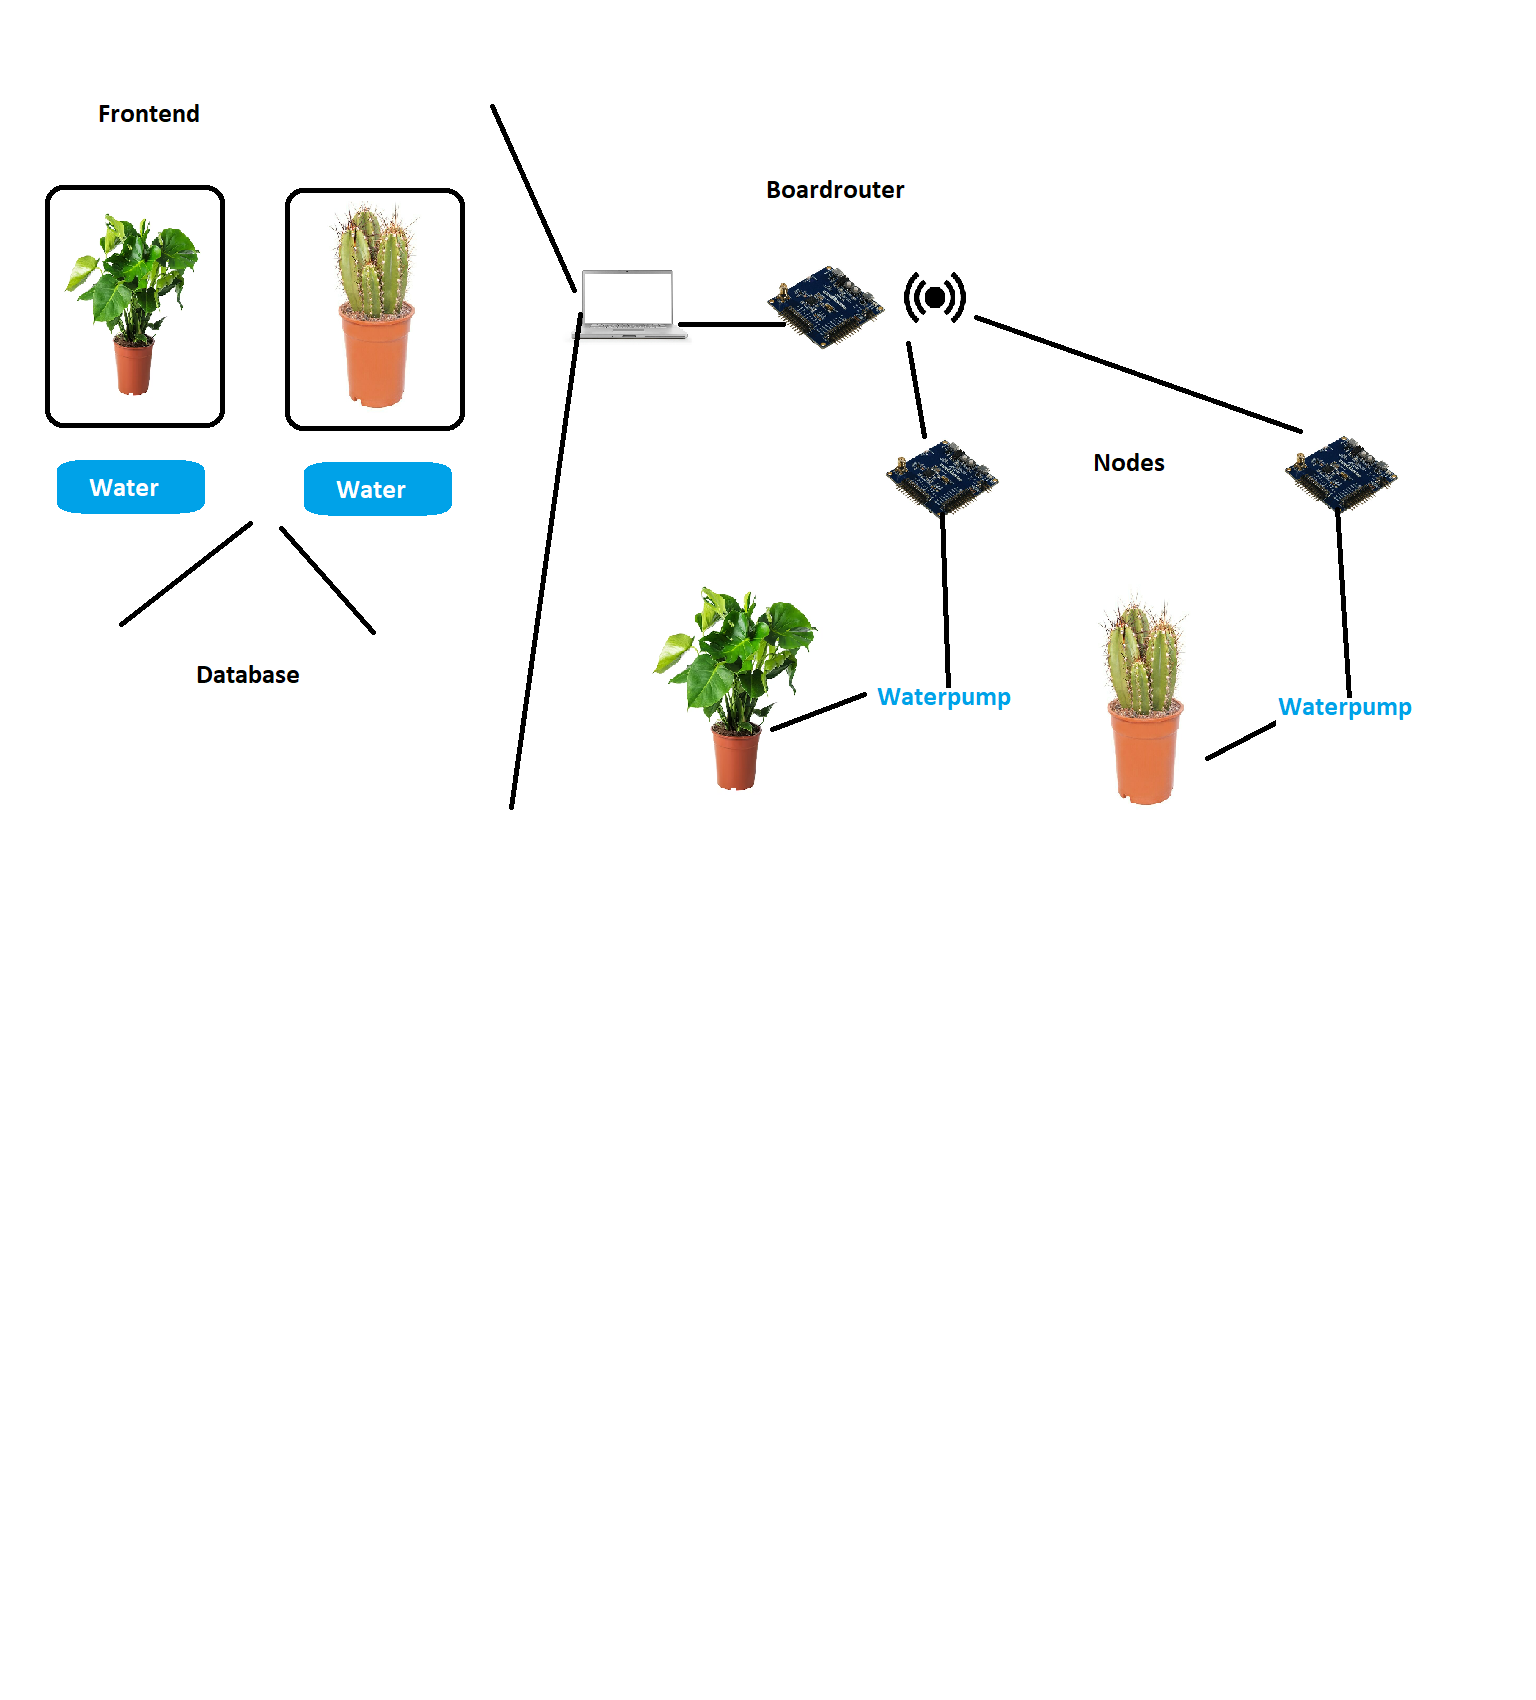
\includegraphics[scale=0.3]{Design_Scheme.png}
\end{frame}

\begin{frame}{short Timeline}
    09.05.2022: Group has formed. Task and Ressources were discussed

    \vspace*{0.25cm}
    
    Getting to know the project. Creating communication and development infrastructure. Thinking about Project Ideas.
    
    \vspace*{0.25cm}

    11.05.2022: Hardware received from Hauke and bought ourselves. HDC1000 Sensor implemented. Started working on the Frontend.
    
    \vspace*{0.25cm}
    
    16.05.2022: Talking about Problems and fixing them. Reorginising Project and development structure. (Communication problems Hardware problems)

    \vspace*{0.25cm}

    Getting to know the Board and thinking about ways to communicate between boards and PC. Working on the sensor and waterpump.

    \vspace*{0.25cm}
    
    23.05.2022: Finding a way to communicate between Boards. Discussing problems and fixing them (HDC1000 not that useful). Getting more Hardware.
    
    \vspace*{0.25cm}
    Implementing Boardrouter. Frontend. Waterpump.
    
    Still some Things to do
    
    
\end{frame}

\begin{frame}
    \frametitle{Hardware}

    \begin{itemize}
        \item Atmel SAMR21 Xplained. \(\leadsto\) One of the available boards from Hauke. We chose this one since we planned to not use Wifi but the more energy efficient IEEE802.15.4.
        \item HDC1000 Temperature and Humidity Sensor, soldered by us.
        \item Soil Moisture Sensor.
        \item Pumps. (ordered from Amazon)
        \item Boards with integrated circuitry for connecting the pumps. (After attempting to build a circuit ourselves)
    \end{itemize}
\end{frame}

\begin{frame}
    \frametitle{Firmware}

    \begin{itemize}
        \item Implemented fetching data from the HDC1000 sensor via the RIOT driver.
        \item The board comes with prebuilt 802.15.4 capabilities, so it is only natural to use low-power radio frequency communication.
        \item Which protocols to use? For 802.15.4, the RIOT documentation only specifies the availability of the GNRC, OpenWSN and OpenThread stacks. We went with the GNRC stack, as the others seemingly implement features we will surely not use. We do not think we will require any other stacks, so this should suffice.
    \end{itemize}
\end{frame}

\begin{frame}
    \frametitle{Boardrouter}

    \begin{itemize}
        \item Board communicates over an USB-connection with Laptop. Several Methods and a lot of problems. One method worked:
        \begin{itemize}
            \item Creating a localnetwork with ethos
            \item able to send packages to HOST and NODES
        \end{itemize}
    \end{itemize}
\end{frame}

\begin{frame}
    \frametitle{Nodes}

    \begin{itemize}
        \item Is able to control the pump
        \item receives packages from BR
    \end{itemize}
\end{frame}

\begin{frame}
    \frametitle{Frontend}
    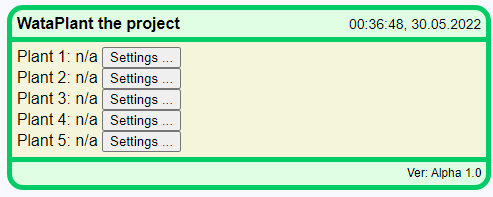
\includegraphics[scale=0.8]{Frontend.png}
    \begin{itemize}
        \item Design
        \item Database
    \end{itemize}
\end{frame}

\begin{frame}
    \frametitle{Improvement}
    \begin{itemize}
        \item Everything is Hardcoded
        \item Can not send or receive package that triggers a function call
        \item Database has to be made or found
        \item Can not send function call from Buttonclick on Frontend
        \item no scalability
    \end{itemize}
\end{frame}

\begin{frame}
    \frametitle{Conclusion}

    \begin{itemize}
        \item Good in Time
        \item A lot of Problems on the way
        \item C is hard
    \end{itemize}
\end{frame}

\end{document}
